\documentclass[xcolor=dvipsnames]{beamer}
\makeatletter\def\Hy@xspace@end{}\makeatother 
\usepackage{graphicx, color, amssymb, amsmath, bm, rotating, graphics,
epsfig, multicol, amsthm}
\usepackage[english]{babel}
\usepackage[T1]{fontenc}
\usepackage[ansinew]{inputenc}
\usepackage[authoryear]{natbib}
%\newcommand{\newblock}{}  %needed to make beamer and natbib play nice
\usepackage{tikz}
\usetikzlibrary{fit}					% fitting shapes to coordinates
\usetheme{Boadilla}
\usecolortheme[named=Red]{structure}
\setbeamercovered{transparent}
\newcommand\ind{\protect\mathpalette{\protect\independenT}{\perp}}
\def\independenT#1#2{\mathrel{\rlap{$#1#2$}\mkern2mu{#1#2}}}
\newcommand\N{\mathcal{N}}
\graphicspath{{../doc/plots/}}
\title[Interweaving MCMC Strats for DLMs]{Interweaving Markov Chain Monte Carlo Strategies for Efficient
Estimation of Dynamic Linear Models}
%\subtitle{}
\author[M. Simpson]{Matthew Simpson}
\date{\today}
\institute[Deps of Stat \& Econ, ISU]{Departments of Statistics and Economics, Iowa State University}


%\title[short title]{long title}
%\subtitle[short subtitle]{long subtitle}
%\author[short name]{long name}
%\date[short date]{long date}
%\institution[short name]{long name}

% very important to use option [fragile] for frames containing code output!

\begin{document}

\begin{frame}
\titlepage
\end{frame}

\begin{frame}
\frametitle{Interweaving: A Motivating Example}
Adapted from \citet{yu2011center}, suppose:
\begin{align*}
y|\theta, \mu & \sim \N(\theta, V) \\
\theta|\mu & \sim \N(\mu, W) 
\end{align*}
with $V$, $W$ known and $p(\mu)\propto 1$.\\~\\
Posterior: $\mu|y \sim \N(y, V+W)$\\~\\
DA algorithm:
\begin{align*}
\theta|\mu,y &\sim \N\left(\frac{V\mu + Wy}{V+W}, \frac{VW}{V+W}\right)\\
\mu |\theta, y &\sim \N(\theta, W)
\end{align*}
\end{frame}

\begin{frame}
\frametitle{Interweaving: A Motivating Example}
Let $\gamma = \theta - \mu$. Then:
\begin{align*}
y|\theta, \gamma & \sim \N(\mu + \gamma, V) \\
\gamma|\mu & \sim \N(0, W) 
\end{align*}
DA algorithm based on $\gamma$:
\begin{align*}
\gamma|\mu,y &\sim \N\left(\frac{W(\mu - y)}{V+W}, \frac{VW}{V+W}\right)\\
\mu |\gamma, y &\sim \N(y-\gamma, V)
\end{align*}
\end{frame}

\begin{frame}
\frametitle{Interweaving: A Motivating Example}
Alternate between two DAs (alternating algorithm):
\begin{align*}
[\theta|\mu,y] \to [\mu|\theta,y] \to [\gamma|\mu,y] \to [\mu|\gamma,y]
\end{align*}
Weave two DAs together (interweaving algorithm):
\begin{align*}
[\theta|\mu,y] \to [\gamma|\theta,y] \to [\mu|\gamma,y]
\end{align*}
Alternate representation:
\begin{align*}
[\theta|\mu,y] \to [\mu|\theta,y] \to [\gamma|\mu,\theta,y] \to [\mu|\gamma,y]
\end{align*}
{\color{blue}The interweaving algorithm obtains IID draws from the posterior of $\mu$.}
\end{frame}

\begin{frame}
  \frametitle{Outline}
  Goal: apply interweaving to DLMs\\~\\
  \begin{enumerate}
    \item Intro to interweaving\\~\\
    \item The model\\~\\
    \item DAs for the model, new and old\\~\\
    \item Simulation results in the local level model
  \end{enumerate}
\end{frame}

\begin{frame}
\frametitle{Global Interweaving Strategy (GIS)}
From \citet{yu2011center}: target posterior distribution $p(\phi|y)$ with two DAs $\theta$ and $\gamma$ such that
\begin{align*}
\int p(\theta,\phi|y) d\theta = p(\phi|y) \ \ \ \ \mbox{and}\ \ \ \int p(\gamma,\phi|y) d\gamma = p(\phi|y) 
\end{align*}
Then:
\begin{align*}
[\theta|\phi,y] \to [\gamma|\theta,y] \to [\phi|\gamma,y]
\end{align*}
or more commonly:
\begin{align*}
[\theta|\phi,y] \to [\phi|\theta,y] \to {\color{blue}[\gamma|\phi,\theta,y]} \to [\phi|\gamma,y]
\end{align*}
\end{frame}

\begin{frame}
\frametitle{Ancillary-Sufficiency Interweaving Strategy (ASIS)}
GIS where one DA is a sufficient augmentation (SA) and the other is an ancillary augmentation (AA).\\~\\
\begin{itemize}
\item$\theta$ is an SA if $p(y|\theta,\phi)=p(y|\theta)$ (AKA centered augmentation)\\~\\
\item$\theta$ is an AA if $p(\theta|\phi)=p(\theta)$ (AKA non-centered augmentation)\\~\\
\end{itemize}
Componentwise Interweaving Strategy (CIS):\\~\\
\begin{itemize}
\item Motivation: Finding an SA--AA pair is often difficult for $\phi=(\phi_1,\phi_2)$, but not for $\phi_1$ and $\phi_2$ separately.\\~\\
\item Basic idea: GIS (or ASIS) for sub-blocks of $\phi$.\\~\\
\item Can use the same DA in multiple sub-blocks of $\phi$.
\end{itemize}
\end{frame}

\begin{frame}
\frametitle{Why interweaving?}
\begin{itemize}
  \item  GIS has a geometric rate of convergence no worse than the worst of the two underlying DA algorithms, and the bound gets better the less $\theta$ and $\tilde{\theta}$ are correlated in the posterior \citep{yu2011center}.\\~\\
  \item If the two DAs are independent in the posterior, then GIS results in {\color{blue}\textit{\textbf{IID}}} draws from the posterior \citep{yu2011center}. \\~\\
  \item Often GIS has better convergence than the associated alternating algorithm.\\~\\
  \item Under weak conditions the ASIS algorithm is the same as the optimal PX-DA algorithm of \citet{liu1999parameter} \citep{yu2011center}.\\~\\
  \item The CIS sampler does at least as well (in some sense) as the Gibbs sampler that integrates out the augmented data vectors \citep{yu2011center}.
  \end{itemize}
\end{frame}

\begin{frame}[fragile]
\frametitle{Interweaving in Time Series Models}
\begin{itemize}
\item \citet{yu2011center} use a time series of Poisson counts to illustrate CIS.\\~
\item \citet{kastner2013ancillarity} use ASIS to improve estimation of the stochastic volatility model. \verb0R0 package: \verb0stochvol0.\\~
\item Lots of relevant work on reparameterization: \\~
\begin{itemize}
\item AR(1) plus noise: \citet{pitt1999analytic}\\~
\item Stochastic volatility models: \citet{shephard1996statistical,fruhwirth2003bayesian,roberts2004bayesian,bos2006inference,strickland2008parameterisation,fruhwirth2008heston}\\~
\item Poisson counts: \citet{fruhwirth2006auxiliary}\\~
\item Dynamic regression: \citet{fruhwirth2004efficient}
\end{itemize}
\end{itemize}
\end{frame}

\begin{frame}[fragile]
  \frametitle{The Dynamic Linear Model} 
  For $t=1,2,...,T$
  \begin{align*}
    y_t  =&F_t\theta_t +  v_t  \qquad \mbox{(observation equation)}\\
    \theta_t =& G_t\theta_{t-1} + w_t \qquad \mbox{(system equation)}
  \end{align*} 
  with $v_t\stackrel{ind}{\sim}\N_k(0,V)$ independent of $w_t\stackrel{ind}{\sim}\N_p(0,W)$.\\~\\

\begin{figure}
  \centering
    \tikzstyle{state}=[circle, thick, minimum size=1.2cm, draw=black!80]
    \tikzstyle{obs}=[circle, thick, minimum size=1.2cm, draw=black!80]
  \begin{tikzpicture}[>=latex,text height=1.5ex,text depth=0.25ex]
    \matrix[row sep=0.5cm,column sep=0.5cm]{
    % First line: Observations
    &
    \node (y_t-1) [obs]{$y_{t-1}$}; &
    &
    \node (y_t) [obs]{$y_{t}$}; &
    &
    \node (y_t+1) [obs]{$y_{t+1}$}; &
    \\
    % Second line: States
    \node (theta_t-2) {$\cdots$}; &
    \node (theta_t-1) [state]{$\theta_{t-1}$}; &
    &
    \node (theta_t) [state]{$\theta_{t}$}; &
    &
    \node (theta_t+1) [state]{$\theta_{t+1}$}; &
    \node (theta_t+2) {$\cdots$}; \\
    };
    
    % The diagram elements are now connected through arrows:
    \path[->]
    (theta_t-2) edge (theta_t-1)
    (theta_t-1) edge (theta_t)
    (theta_t) edge (theta_t+1)
    (theta_t+1) edge (theta_t+2)
    (theta_t-1) edge (y_t-1)
    (theta_t) edge (y_t)
    (theta_t+1) edge (y_t+1)
    ;
  \end{tikzpicture}
  \end{figure}

For convenience define $y\equiv(y_1',\cdots,y_T')'$ and $\theta\equiv(\theta_0',\cdots,\theta_T)'$.

\end{frame}

\begin{frame}
  \frametitle{The Dynamic Linear Model} 
Define 
\begin{align*}
H_t &= G_tG_{t-1}\cdots G_1\\ 
K_t &= I_p + G_t + G_tG_{t-1} + \cdots + G_tG_{t-1}\cdots G_2\\ 
D_t &= F_tG_tG_{t-1}\cdots G_1.
\end{align*} Then let $\tilde{V}=I_T\otimes V$ and $D$ be block diagonal with elements $D_1,\ldots,D_T$, 
\begin{align*}
\tilde{W}_{Tk\times Tk} &= \begin{bmatrix} K_1'F_1' & K_2'F_2' & \cdots K_T'F_T' \end{bmatrix}' W \begin{bmatrix} K_1'F_1' & K_2'F_2' & \cdots K_T'F_T' \end{bmatrix}, &\\
\tilde{C}_{Tk\times Tk} &= \begin{bmatrix} H_1'F_1' & H_2'F_2' & \cdots H_T'F_T' \end{bmatrix}' C_0 \begin{bmatrix} H_1'F_1' & H_2'F_2' & \cdots H_T'F_T' \end{bmatrix},&
\end{align*}
and $\tilde{m}_{Tp\times 1} = (m_0', m_0', \cdots m_0')'$\\~\\

Marginal model for $y$: 
\begin{align*}
  y|V,W \stackrel{ind}{\sim} N_{Tk}(D\tilde{m}, \tilde{V} + \tilde{W} + \tilde{C})
\end{align*}
\end{frame}

\begin{frame}
  \frametitle{The Dynamic Linear Model} 
Let $\phi$ denote the unknown parameter. Potentially $F_t(\phi)$ and $G_t(\phi)$, but for simplicity assume $\phi=(V,W)$.\\~\\

Priors: independently assume \\~\\
\begin{itemize}
\item[]$\theta_0\sim \N_p(m_0,C_0)$, $V\sim IW(\Lambda_V,\lambda_V)$, and $W\sim IW(\Lambda_W,\lambda_W)$\\~\\
\end{itemize}

Then $p(\phi|y)\propto$
\begin{align*}
p(\phi)|\tilde{V} + \tilde{W} + \tilde{C}|^{-1/2}\exp\left[-\frac{1}{2}\left(y-D\tilde{m}\right)'(\tilde{V} + \tilde{W} + \tilde{C})^{-1}\left(y-D\tilde{m}\right)\right]
\end{align*}
\end{frame}

\begin{frame}
\frametitle{Data Augmentations for the DLM}
Standard DA: states $\theta$. In terms of $\theta$, the model is:
\begin{align*}
y_t|\theta,V,W \stackrel{ind}{\sim} & \N_k(F_t\theta_t,V)\\ 
\theta_t|\theta_{0:(t-1)},V,W \sim & \N_p(G_t\theta_{t-1},W)
\end{align*} 
{\color{blue}$\theta$ is an SA for $W|V$ and an AA for $V|W$.}\\~\\

Scaled disturbances $\gamma\equiv(\gamma_0',\cdots,\gamma_T)'$ \citep{fruhwirth2004efficient}.
\begin{itemize}
\item[]$\gamma_0=\theta_0$ and $\gamma_t=L_W^{-1}(\theta_t - G_t\theta_{t-1})=L_W^{-1}w_t$ where $L_W$ is the Cholesky decomposition of $W$.
\end{itemize}
Let $\theta_0(\gamma,W)=\gamma_0$ and $\theta_t(\gamma,W)=L_W\gamma_t + G_t\theta_{t-1}(\gamma,W)$. Then:
\begin{align*}
y_t|\gamma,V,W \stackrel{ind}{\sim} & \N_k(F_t\theta_t(\gamma,W),V) \\
\gamma_t|V,W \stackrel{iid}{\sim} & \N_p(0,I_p)
\end{align*} 

{\color{blue}$\gamma$ is an AA for $(V,W)$.}

\end{frame}

\begin{frame}
\frametitle{New Data Augmentations for the DLM}
Scaled errors $\psi\equiv(\psi_0',\cdots,\psi_T')'$:
\begin{itemize}
\item[]$\psi_0=\theta_0$ and $\psi_t=L_V^{-1}(y_t - F_t\theta_t)=L_V^{-1}v_t$ where $L_V$ is the Cholesky decomposition of $V$.
\end{itemize}
For convenience, assume $F_t$ is square and invertible for all $t$.
 
\ \ (So $dim(y_t)=dim(\theta_t)$.)\\~

In terms of $\psi$ the model is:
\begin{align*}
y_t|\psi,V,W \stackrel{ind}{\sim} &\N_p(\mu_t(\psi,V),F_tWF_t')\\
\psi_t|V,W \stackrel{iid}{\sim} &\N_p(0,I_p)
\end{align*} 
where $\mu_t(\psi,V)$ is complicated.\\~\\

{\color{blue}$\psi$ is an AA for $(V,W)$.}
\end{frame}

\begin{frame}
\frametitle{New Data Augmentations for the DLM}
Wrongly-scaled disturbances $\tilde{\gamma}\equiv(\tilde{\gamma}_0',\cdots,\tilde{\gamma}_T')'$:
\begin{itemize}
\item[]$\tilde{\gamma}_0=\theta_0$ and $\tilde{\gamma}_t=L_V^{-1}(\theta_t - G_t\theta_{t-1})=L_V^{-1}w_t$
\end{itemize}
\begin{align*}
  y_t|\tilde{\gamma},V,W \stackrel{ind}{\sim} \N_p\left(F_t\theta_t(\tilde{\gamma},V), V\right), \qquad 
  \tilde{\gamma}_t \stackrel{ind}{\sim} \N_p(0,L_V^{-1}W(L_V^{-1})')
\end{align*}
where $\theta_0(\tilde{\gamma},V)=\tilde{\gamma}_0$ and $\theta_t(\tilde{\gamma},V) = L_V\tilde{\gamma}_t + G_t\theta_{t-1}(\tilde{\gamma},V)$.\\~\\

Wrongly-scaled errors $\tilde{\psi}\equiv(\tilde{\psi}_0',\cdots,\tilde{\psi}_T')'$:
\begin{itemize}
\item[]$\tilde{\psi}_0=\theta_0$ and $\tilde{\psi}_t=L_W^{-1}(y_t - F_t\theta_{t})=L_W^{-1}v_t$
\end{itemize}
\begin{align*}
  y_t|V,W,\tilde{\psi},y_{1:t-1} \sim \N_p(\tilde{\mu}_t(\tilde{\gamma},W), F_tWF_t'), \qquad
  \tilde{\psi}_t  \stackrel{iid}{\sim} \N_p(0,L_W^{-1}V(L_W^{-1})')
\end{align*}
where $\tilde{\mu}_t(\tilde{\gamma},W)$ is complicated.\\~\\

{\color{blue} $\tilde{\gamma}$ is an SA for $W|V$ and $\tilde{\psi}$ is an SA for $V|W$.}
\end{frame}

\begin{frame}
\frametitle{The Elusive Search for an SA}
Suppose $\eta$ is an SA for the DLM such that
\begin{align*}
 \left. \begin{bmatrix}\eta \\ y \end{bmatrix}\right|\phi \sim N\left(\begin{bmatrix} \alpha_\eta \\ D\tilde{m} \end{bmatrix}, \begin{bmatrix}
   \Omega_\eta & \Omega_{y,\eta}' \\
   \Omega_{y,\eta} & \tilde{V} + \tilde{W} + \tilde{C} \end{bmatrix}\right).
\end{align*}
Then $\tilde{\eta}=\Omega_{y,\eta}'\Omega_{\eta}^{-1}\eta$ is also an SA and
\[
\tilde{\eta}|\phi \sim N(A\alpha_{\eta},\tilde{V} + \tilde{W} + \tilde{C} - \Sigma)
\]
where $A=\Omega_{y,\eta}'\Omega_{\eta}^{-1}$, $\Sigma = \tilde{V} + \tilde{W} + \tilde{C} - \Omega_{y,\eta}\Omega_{\eta}^{-1}\Omega_{y,\eta}'$ and $\alpha_{\eta}$ are functionally independent of $\phi$ and the conditional posterior of $\phi$ given $\tilde{\eta}$ can be written as
\begin{align*}
&p(\phi|\tilde{\eta},y) \propto p(\phi)|\tilde{V} + \tilde{W} + \tilde{C} - \Sigma|^{-1/2}\\
&\times \exp\left[-\frac{1}{2}(\tilde{\eta} - A\alpha_{\eta})'(\tilde{V} + \tilde{W} + \tilde{C} - \Sigma)^{-1}(\tilde{\eta} - A\alpha_{\eta})\right].
\end{align*}
\end{frame}

\begin{frame}
\frametitle{The Elusive Search for an SA}
The conditional posterior of $\phi$ given $\eta$ is difficult to characterize:
\begin{align*}
p(\phi|\eta,y) \propto  p(\phi) |\Omega_{\eta}|^{-1/2}\exp\left[-\frac{1}{2}(\eta-\alpha_{\eta})\Omega_{\eta}^{-1}(\eta-\alpha_{\eta})\right]
\end{align*}
When $(A'A)$ is invertible:
\begin{align*}
p(\phi|&\eta,y) \propto p(\phi) |(A'A)^{-1}A'(\tilde{V} + \tilde{W} + \tilde{C} - \Sigma)A(A'A)^{-1}|^{-1/2}\\
&\times \exp\left[-\frac{1}{2}(\eta - \alpha_{\eta})'(A'A)^{-1}A'(\tilde{V} + \tilde{W} + \tilde{C} - \Sigma)A(A'A)^{-1}(\eta - \alpha_\eta)\right]
\end{align*}
\\~\\
Upshot: hard to find a SA for $(V,W)$.

\end{frame}

\begin{frame}
\frametitle{MCMC Strategies}
The standard DA Algorithm--the state sampler: {\color{blue}$[\theta|V,W,y] \to [V,W|\theta,y]$}
\begin{itemize}
\item $p(\theta|V,W,y)$ is Gaussian --- draw using the mixed Cholesky factor algorithm (MCFA) \citep{mccausland2011simulation}.
\item Conditional on $(\theta,y)$, $V$ and $W$ are independent inverse Wishart.\\~\\
\end{itemize}

Scaled disturbance sampler: {\color{blue}$[\gamma|V,W,y] \to [V|W,\gamma,y] \to [W|V,\gamma,y]$}
\begin{itemize}
\item $p(\gamma|V,W,y)$ is Gaussian, but easier to draw $\theta$ using MCFA and transform.
\item $p(V,W|\gamma,y)$ is complicated, but $p(V|W,\gamma,y)$ is inverse Wishart.
\item $p(W|V,\gamma,y)$ is still complicated, but less so.
\end{itemize}
\end{frame}

\begin{frame}
\frametitle{MCMC Strategies}
Scaled error sampler: {\color{blue}$[\psi|V,W,y] \to [V|W,\psi,y] \to [W|V,\psi,y]$}
\begin{itemize}
\item $p(\psi|V,W,y)$ is Gaussian and can use MCFA directly.
\item $p(V,W|\psi,y)$ is complicated, but $p(V|W,\psi,y)$ is less complicated. 
\item $p(W|V,\psi,y)$ is inverse Wishart.\\~\\
\end{itemize}

Wrongly-scaled samplers are analogous to their correctly-scaled counterparts.\\~\\

Alternating and GIS easy to construct once sampling from the difficult densities is accomplished.
\end{frame}

\begin{frame}
\frametitle{MCMC Strategies}
CIS sampler: 
\begin{itemize}
\item $\gamma$ is an AA and $\tilde{\gamma}$ is an SA for $W|V$.
\item $\psi$ is an AA and $\tilde{\psi}$ is an SA for $V|W$.
\end{itemize}
So:
\begin{align*}
&[\psi|V,W,y]\to[V|W,\psi,y]\to{\color{blue}[\tilde{\psi}|V,W,\psi,y]}\to[V|W,\tilde{\psi},y]\to\\
&{\color{blue}[\tilde{\gamma}|V,W,\tilde{\psi},y]}\to[W|V,\tilde{\gamma},y]\to{\color{blue}[\gamma|V,W,\tilde{\gamma},y]}\to[W|V,\gamma,y]
\end{align*}
But this is equivalent to:
\begin{align*}
&[\psi|V,W,y]\to[V|W,\psi,y]\to{\color{blue}[\theta|V,W,\psi,y]}\to[V|W,\theta,y]\to\\
&[W|V,\theta,y]\to{\color{blue}[\gamma|V,W,\theta,y]}\to[W|V,\gamma,y]
\end{align*}
Steps of this sampler can be rearranged to obtain the SE-SD GIS sampler:
\begin{align*}
&[\psi|V,W,y]\to[V|W,\psi,y]\to[W|V,\psi,y]\to\\
&{\color{blue}[\gamma|V,W,\psi,y]}\to[V|W,\gamma,y]\to[W|V,\gamma,y]
\end{align*}

\end{frame}

\begin{frame}[fragile]
\frametitle{Evaluating the Strategies: the Local Level Model}
Model: for $t=1,2,...,T$
\begin{align*}
    y_t|\theta  \stackrel{ind}{\sim}&\N_1(\theta_t,V) \qquad (\mbox{observation equation})\\
    \theta_t|\theta_{0:(t-1)} \sim& \N_1(\theta_{t-1},W) \qquad (\mbox{system equation})
  \end{align*} 

Then $p(W|V,\gamma,y)$ and $p(V|W,\psi,y)$ have the form:
\begin{align*}
p(x)\propto x^{-\alpha-1}\exp\left[ -ax + b\sqrt{x} -c/x\right], \qquad a,c,\alpha,x>0, b\in\Re
\end{align*}
Similarly $p(W|V,\tilde{\psi},y)$ and $p(V|W,\tilde{\gamma},y)$ have the form:
\begin{align*}
p(y)\propto y^{-\alpha-1}\exp\left[ -ay + b/\sqrt{y} -c/y\right], \qquad a,c,\alpha,y>0, b\in\Re
\end{align*}
Rejection sampling with a Cauchy proposal works for $\log(x)$ and $\log(y)$.\\~\\

Often $p(x)$ is log concave $\to$ adaptive rejection sampling (\verb0R0 package \verb0ars0).
\end{frame}

\begin{frame}
\frametitle{Evaluating the Strategies: LLM - Simulation Setup}

Let $V^*$ and $W^*$ denote the true values used to simulate the time series.\\~\\

Independent priors:
\begin{itemize}
\item $\theta_0\sim N(0, 10^7)$, $V\sim IG(5, 4V^*)$ and $W\sim IG(5, 4W^*)$.\\~\\
\end{itemize}

Simulation Setup:
\begin{itemize}
\item Simulated data: $T=10$, $T=100$ \& $T=1000$ and $V^*$, $W^*$ $=10^{i/2}$ with $i=-4,-3,\cdots,4$.
\item Each sampler was used to fit the model to each dataset using one Markov chain started at $(V^*,W^*)$.
\end{itemize}

\end{frame}


\begin{frame}
\frametitle{LLM Results --- ESP for T=10}
\centering
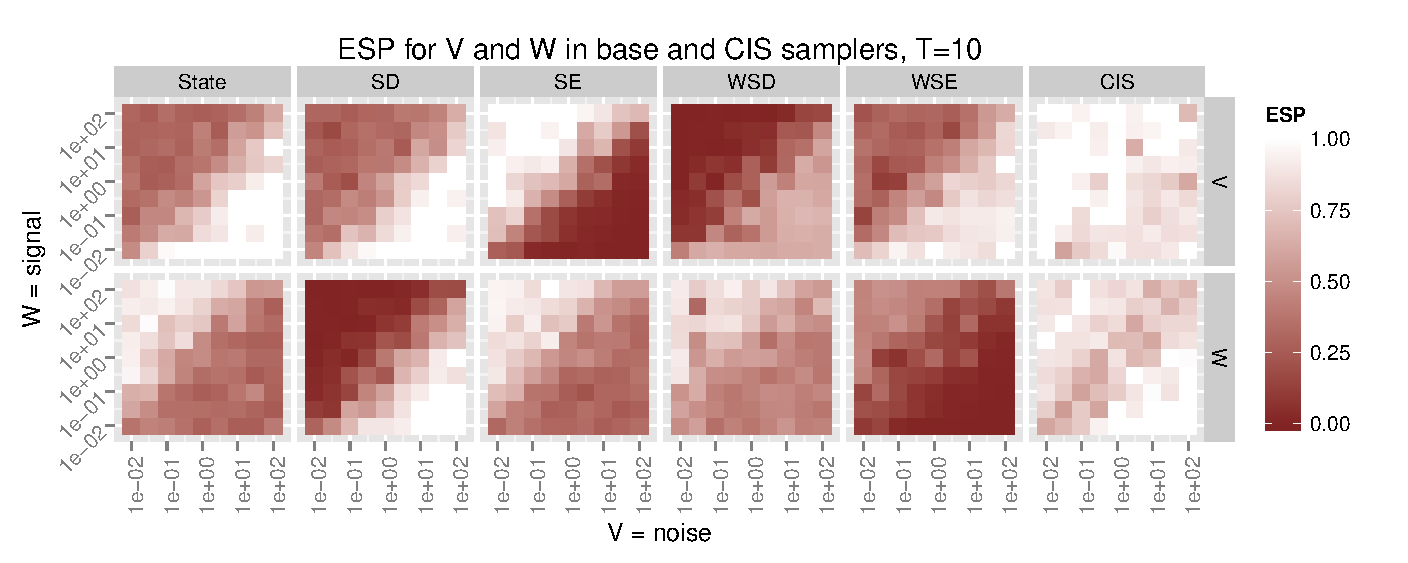
\includegraphics[width=0.75\textwidth]{basecisESplot10}\\
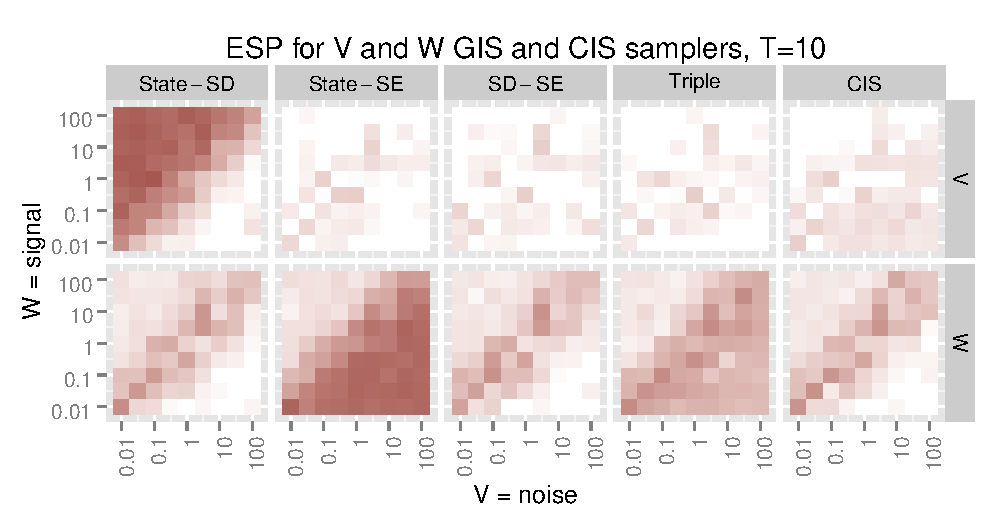
\includegraphics[width=0.49\textwidth]{altintESplotV10}
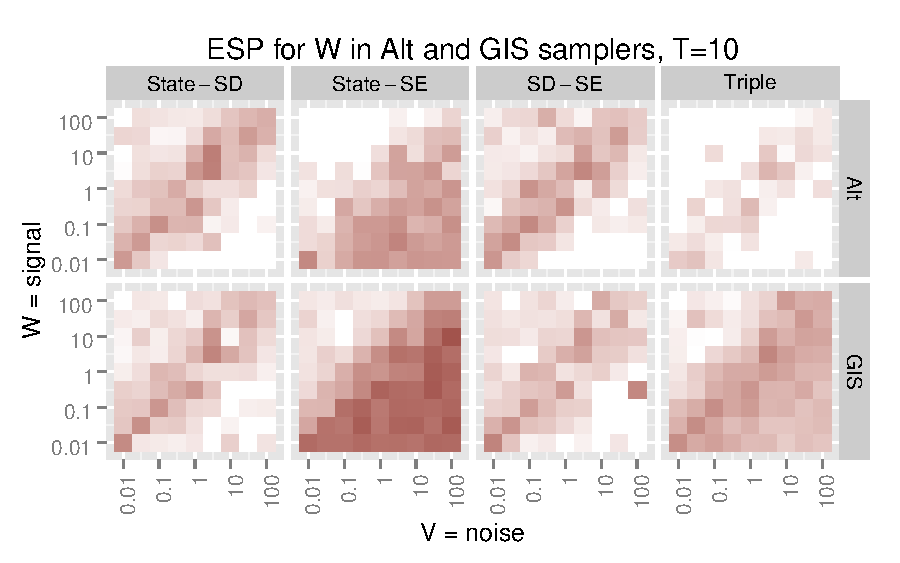
\includegraphics[width=0.49\textwidth]{altintESplotW10}
\end{frame}

\begin{frame}
\frametitle{LLM Results --- ESP for T=100}
\centering
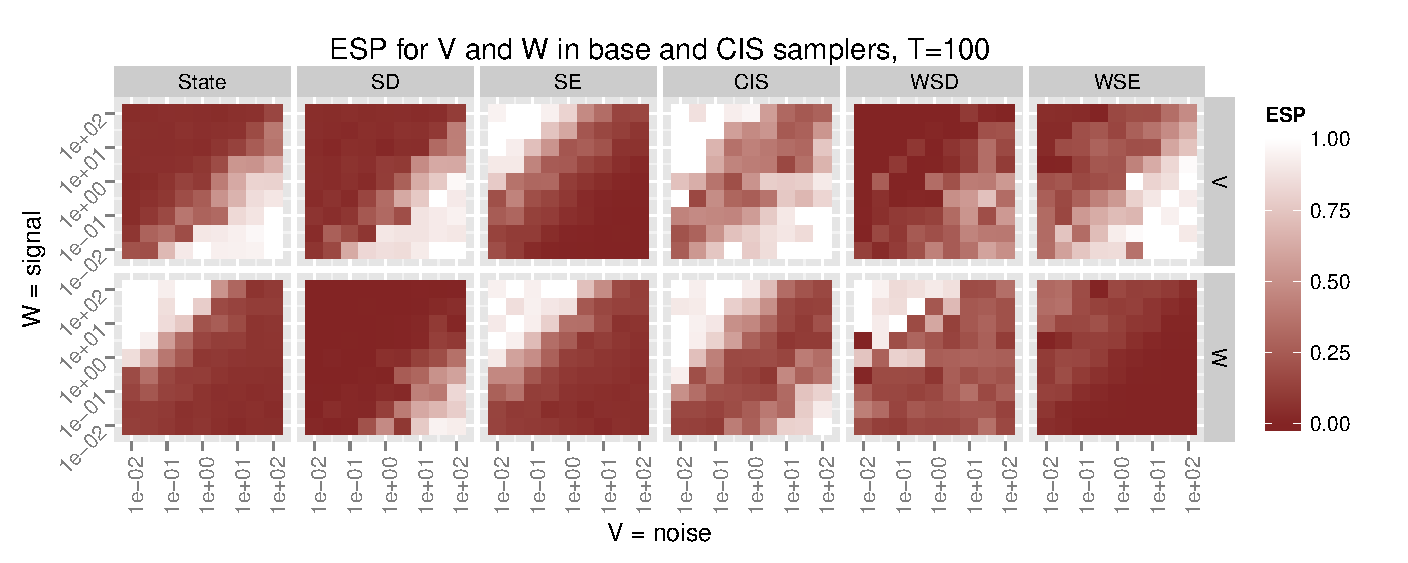
\includegraphics[width=0.75\textwidth]{basecisESplot100}\\
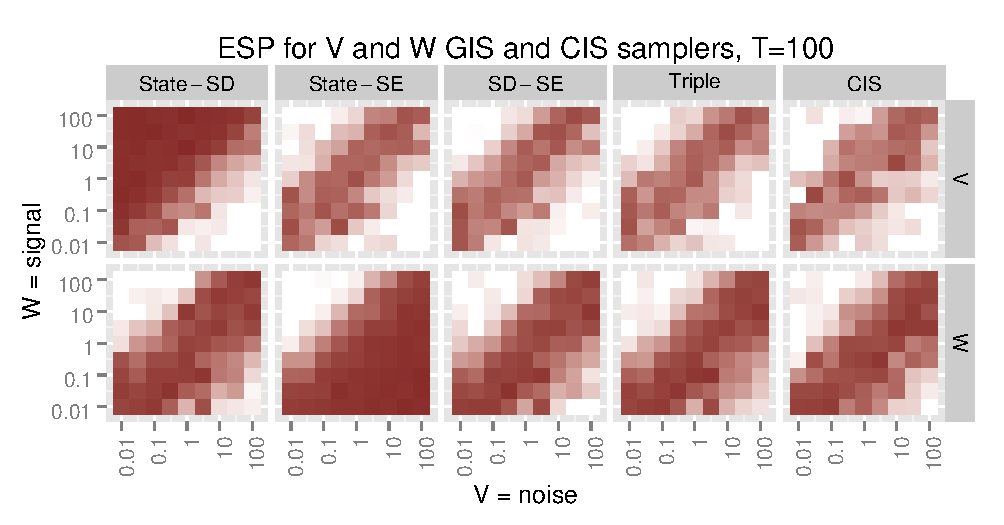
\includegraphics[width=0.49\textwidth]{altintESplotV100}
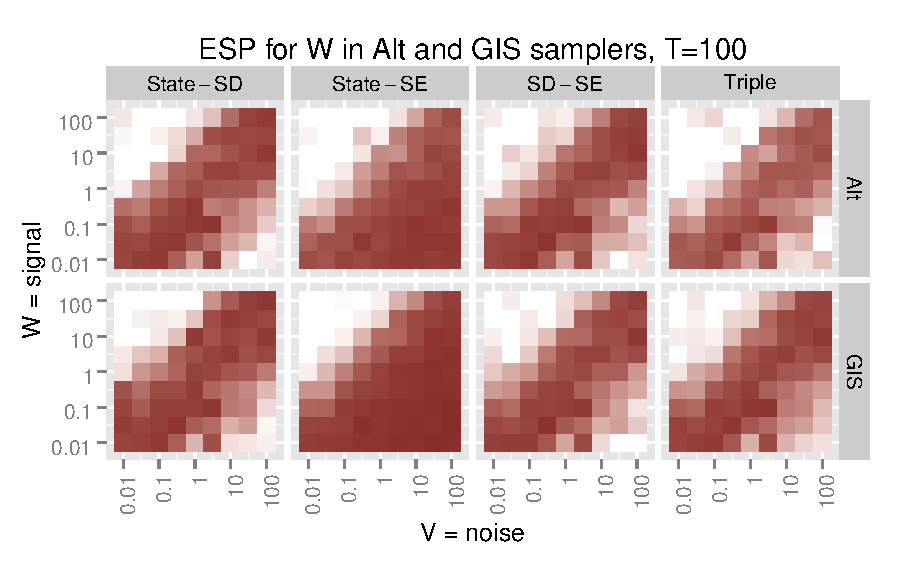
\includegraphics[width=0.49\textwidth]{altintESplotW100}
\end{frame}

\begin{frame}
\frametitle{LLM Results --- ESP for T=1000}
\centering
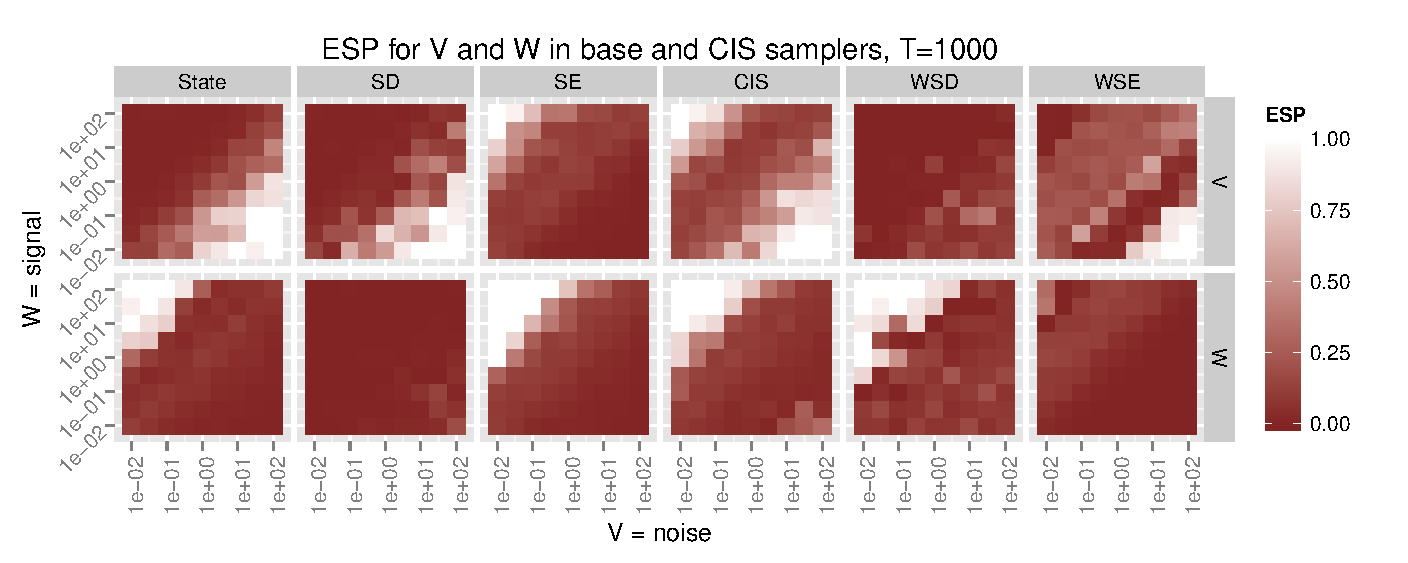
\includegraphics[width=0.75\textwidth]{basecisESplot1000}\\
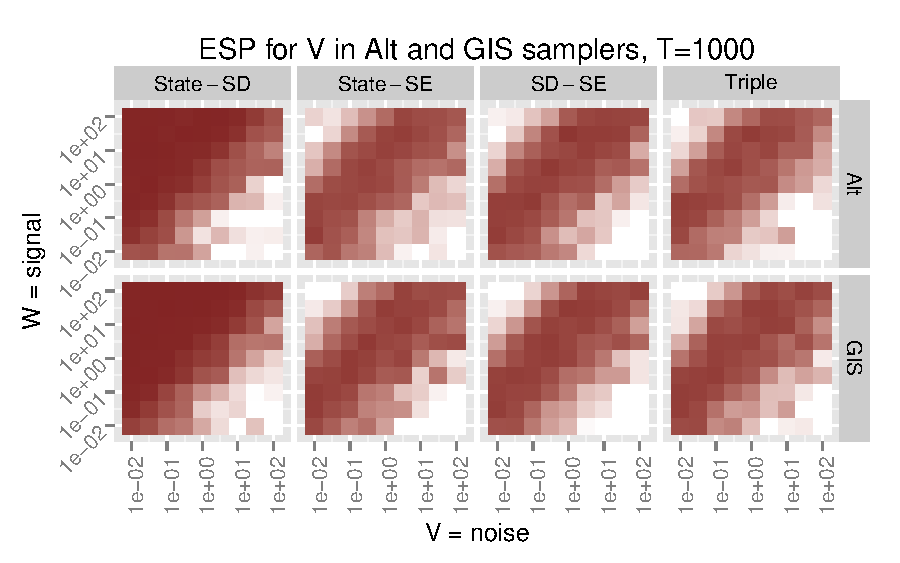
\includegraphics[width=0.49\textwidth]{altintESplotV1000}
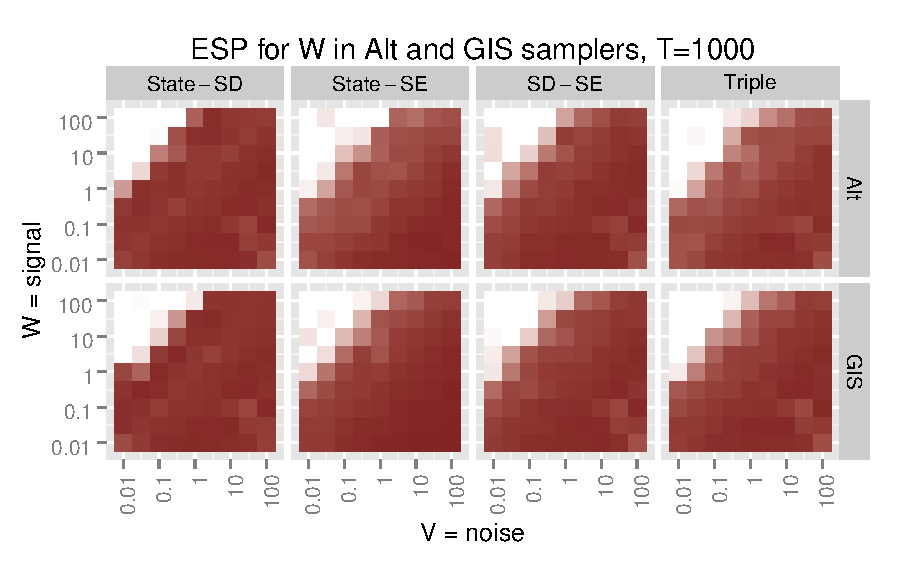
\includegraphics[width=0.49\textwidth]{altintESplotW1000}
\end{frame}

\begin{frame}
\frametitle{LLM Results --- ESP summarized}
Rule of thumb for when each base algorithm has a high ESP for each variable as a function of the true signal-to-noise ratio, $R^*=W^*/V^*$. \\~\\~\\
 \begin{center}
  \begin{tabular}{lccccc}\hline
    Parameter & State & SD & SE & WSD & WSE \\\hline
    V & $R^* < 1$ & $R^* < 1$ & $R^* > 1$ & $R^* < 1$ & $R^* < 1$\\
    W & $R^* > 1$ & $R^* < 1$ & $R^* > 1$ & $R^* > 1$ & $R^* > 1$ \\
      &           &          &           &           &           \\\hline
    Parameter & State-SD        & State-SE       & SD-SE        & Triple            & CIS \\\hline
    V         & $R^* < 1$           & $R^* \not\approx 1$ & $R^* \not\approx 1$ & $R^* \not\approx 1$ & $R^* \not\approx 1$ \\
    W         & $R^* \not\approx 1$ & $R^* > 1$           & $R^* \not\approx 1$ & $R^* \not\approx 1$ & $R^* \not\approx 1$\\\hline
  \end{tabular}
\end{center}\\~\\~\\

Note that as the length of the time series increases, the farther away from one $R^*$ has to be for the sampler to have a high ESP.

\end{frame}

\begin{frame}
\frametitle{LLM Results - log time (minutes) per 1000 effective draws}
\centering
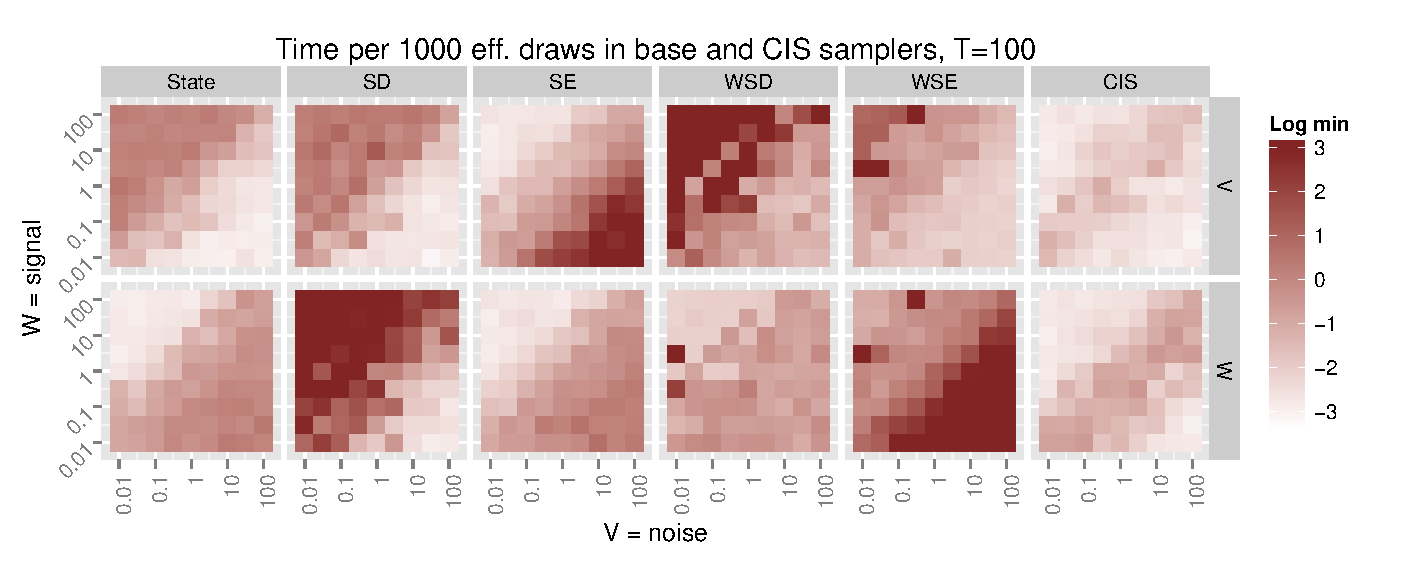
\includegraphics[width=0.75\textwidth]{basecistimeplot100}\\
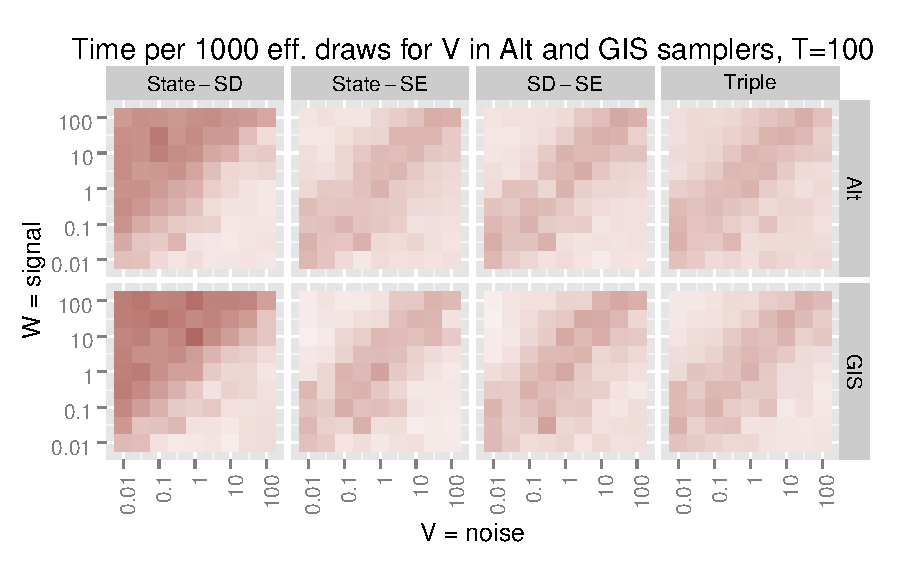
\includegraphics[width=0.49\textwidth]{altgisVtimeplot100}
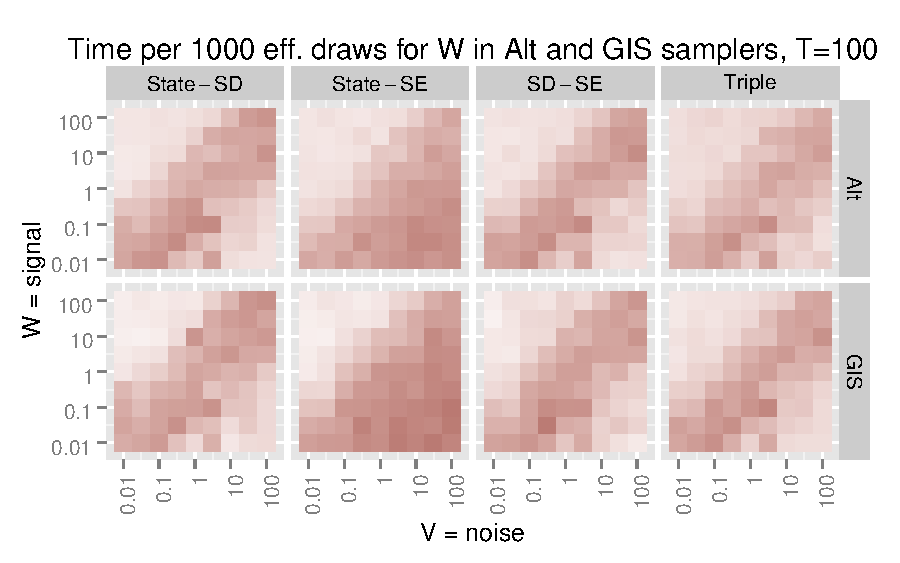
\includegraphics[width=0.49\textwidth]{altgisWtimeplot100}
\end{frame}

\begin{frame}[allowframebreaks]
        \frametitle{References}
        \bibliographystyle{plainnat}
        \bibliography{../doc/dlmasis}
\end{frame} 



\end{document}





\citet{fruhwirth2004efficient} uses the analogue of $\gamma_{0:T}$ in a dynamic regression model.




\begin{frame}
  \frametitle{Effective Sample Size and Effective Sample Proportion}
  Suppose we want to estimate $\mathrm{E}[V|y_{1:T}]$ with 
  \[
  \bar{V}\equiv\frac{\textstyle\sum_{k=1}^KV^{(k)}}{K}
  \]
  If we had $K$ iid draws from the posterior, the CLT would give 
  \[
  \mathrm{Var}(\bar{V})=\frac{\sigma_V^2}{K}
  \]
where $\sigma_V^2=\mathrm{Var}(V|y_{1:T})$. For our markov chain 
\[
\mathrm{Var}(\bar{V})=\frac{\sigma^2_V}{ESS}
\]
where $ESS$ is the ``effective sample size.'' $ESS$ is estimated by fitting an $AR(p)$ model to the chain (to estimate the spectral density at 0). \\~\\
  
  The effective sample proportion is the effective sample size as a proportion of the actual sample size, i.e. $ESP=ESS/K$.
\end{frame}

\begin{frame}
  \frametitle{Simulation Results for the Base Algorithms, $T=10$}
  
\end{frame}

\begin{frame}
    \frametitle{Simulation Results for the Base Algorithms, $T=1000$}

\end{frame}

\begin{frame}
  \frametitle{Takeaways from Base Algorithm Simulations}
  When the signal-to-noise ratio ($W/V$) is low ($<1$), the scaled disturbance sampler has high $ESP$ for both $V$ and $W$; when it's high ($>1$), the scaled disturbance sampler has low $ESP$ for both $V$ and $W$.\\~\\
  
  When the signal-to-noise ratio ($W/V$) is low ($<1$), the scaled error sampler has high $ESP$ for both $V$ and $W$; when it's high ($>1$), the scaled error sampler has low $ESP$ for both $V$ and $W$.\\~\\
  
  The state sampler agrees with the scaled disturbance sampler about $V$ and with the scaled error sampler about $W$. It's at it's best for $(V,W)$ when the signal-to-noise ratio is near $1$.\\~\\
  
  Despite not being an SA-AA pair, $\gamma_{0:T}$ and $\psi_{0:T}$ make a nice beauty and the beast pair.
  
\end{frame}


\begin{frame}
  \frametitle{GIS and Alternating Algorithms for the Local Level Model}
There are four possible GIS algorithms and four corresponding alternating algorithms:
\begin{table}[h]
  \centering
  \scalebox{.9}{
  \begin{tabular}{|l|cccc|}\hline
    Alternating: & State + Dist & State + Error & Dist + Error & Triple\\
    GIS: & State + Dist & State + Error & Dist + Error & Triple\\
    \hline
  \end{tabular}
  }
  \label{table:sams}
\end{table}
\pause

The State-Dist interweaving sampler, for example:
\begin{enumerate}
  \item Draw $\theta_{0:T}$ from $p(\theta_{0:T}|V^{(k)},W^{(k)},y_{1:T})$ using FFBS.
  \item Draw $(V,W)$ from $p(V,W|\theta_{0:T}, y_{1:T})$.
  \item Update $\gamma_{0:T}$ using $\theta_{0:T}$ and $(V,W)$.
  \item Draw $V^{(k+1)}$ from $p(V|\gamma_{0:T}, W, y_{1:T})$.
  \item Draw $W^{(k+1)}$ from $p(W|\gamma_{0:T}, V^{(k+1)}, y_{1:T})$, i.e. the same difficult density from before.\\~\\
\end{enumerate}
\pause
  The State-Dist alternating sampler would replace step 3 with a draw from $p(\gamma_{0:T}|V,W,y_{1:T})$.
\end{frame}

\begin{frame}
    \frametitle{Simulation Results for the GIS Algorithms, $T=10$}
    
\end{frame}

\begin{frame}
    \frametitle{Simulation Results for the GIS Algorithms, $T=10$}
    
\end{frame}

\begin{frame}
    \frametitle{Simulation Results for the GIS Algorithms, $T=1000$}
    
\end{frame}

\begin{frame}
    \frametitle{Simulation Results for the GIS Algorithms, $T=1000$}
    
\end{frame}

\begin{frame}
  \frametitle{Takeaways from GIS Algorithm Simulations}
  For $T$ large enough, alternating or interweaving doesn't make a difference for ESP (but interweaving is less computationally expensive).\\~\\
  
  The Dist-Error interweaving algorithm and the Triple interweaving algorithm appear to have identical ESPs.\\~\\
\pause  
  The ``beauty and the beast'' intuition works for any given parameter, i.e. for $W$, the Dist-Error and State-Dist algorithms have the best ESP, but the State-Error algorithms has worse ESP in some regions of the parameter space.\\~\\
  
  For the reasonable areas of the parameter space ($W/V$ not too small or large), there are still major mixing problems.
\end{frame}

\begin{frame}
  \frametitle{Partial CIS for the Local Level Model}
  Recall $\theta_{0:T}$ is SA for $W|V$ and both $\gamma_{0:T}$ and $\psi_{0:T}$ are AA for $(V,W)$. So all we need is a SA for $V|W$ for a CIS algorithm.\\~\\
\pause  
  This appears hard to find at first glance, instead we can try partial CIS, i.e. an algorithm which only interweaves in one of the Gibbs steps:
  \begin{enumerate}
  \item Draw $\theta_{0:T}$ from $p(\theta_{0:T}|V^{(k)},W^{(k)},y_{1:T})$ using FFBS.
  \item Draw $V^{(k+1)}$ from $p(V|W^{(k)},\theta_{0:T},y_{1:T})$
  \item Draw $W$ from $p(W|V^{(k+.5)},\theta_{0:T},y_{1:T})$
  \item Update $\gamma_{0:T}$ where $\gamma_0=\theta_0$ and $\gamma_t=(\theta_t-\theta_{t-1})/\sqrt{W}$.
  \item Draw $W^{(k+1)}$ from $p(W|V^{(k+1)},\gamma_{0:T},y_{1:T})$\\~\\
  \end{enumerate}
  Note that we have to use $\gamma_{0:T}$ in step 4, otherwise steps 5 and 3 would be identical draws because $p(W|V,\theta_{0:T},y_{1:T})=p(W|V,\psi_{0:T},y_{1:T})$.
\end{frame}

\begin{frame}
  \frametitle{Full CIS for the Local Level Model}
  For $t=1,2,...,T$ define
  \begin{align*}
    \tilde{\gamma}_t & = \frac{\sqrt{W}}{\sqrt{V}}\gamma_t = \frac{\theta_t - \theta_{t-1}}{\sqrt{V}} = \frac{w_t}{\sqrt{V}}\\
  \end{align*}
  with $\tilde{\gamma}_0=\gamma_0=\theta_0$.\\~\\
  \pause
  
  The model written in terms of $\tilde{\gamma}_{0:T}$ is
  \begin{align*}
  y_t|\tilde{\gamma}_{0:T}, V, W &\stackrel{ind}{\sim} N(\tilde{\gamma}_0 + \sqrt{V}\textstyle\sum_{s=1}^{t-1}\tilde{\gamma}_s, V)\\
  \tilde{\gamma}_t|V,W &\stackrel{iid}{\sim} N(0, W/V)
\end{align*}
So $\gamma_{0:T}$ \& $\tilde{\gamma}_{0:T}$ make a AA-SA pair for $W|V$
\end{frame}


\begin{frame}
  \frametitle{Full CIS for the Local Level Model}
  For $t=1,2,...,T$ define
  \begin{align*}
    \tilde{\psi}_t & = \frac{\sqrt{V}}{\sqrt{W}}\psi_t = \frac{y_t - \theta_{t}}{\sqrt{W}} = \frac{v_t}{\sqrt{W}}\\
  \end{align*}
  with $\tilde{\psi}_0=\psi_0=\theta_0$.\\~\\
  \pause
  
  The model written in terms of $\tilde{\psi}_{0:T}$ is
  \begin{align*}
  y_t|\tilde{\psi}_{0:T}, y_{0:t-1}, V, W & \sim N(y_{t-1} + \sqrt{W}(\tilde{\psi}_t - \tilde{\psi}_{t-1}), W)\\
  \tilde{\psi}_t|V,W &\stackrel{iid}{\sim}N(0,V/W)
\end{align*}
except for $t=1$, the mean of the system equation is $\sqrt{W}\tilde{\psi}_1 - \tilde{\psi}_0$.\\~\\

So $\psi_{0:T}$ \& $\tilde{\psi}_{0:T}$ make a AA-SA pair for $V|W$
\end{frame}

\begin{frame}
    \frametitle{Full CIS for the Local Level Model}
It turns out that
\begin{align*}
  p(W|\tilde{\gamma}_{0:T}, V, y_{1:T}) &= p(W|\theta_{0:T}, V, y_{1:T})\\
  p(V|\tilde{\psi}_{0:T}, W, y_{1:T}) &= p(V|\theta_{0:T}, W, y_{1:T})
\end{align*}
\pause 
which makes full CIS look like an extention of partial CIS:
\begin{enumerate}
  \item Draw $\theta_{0:T}$ from $p(\theta_{0:T}|V^{(k)},W^{(k)},y_{1:T})$.
  \item Draw $V$ from $p(V|W^{(k)}, \theta_{0:T}, y_{1:T})$.
  \item Update $\psi_{0:T}$ from $V$ and $\theta_{0:T}$.
  \item Draw $V^{(k+1)}$ from $p(V|W^{(k)}, \psi_{0:T}, y_{1:T})$.
  \item Update $\theta_{0:T}$ from $V^{(k+1)}$ and $\psi_{0:T}$.
  \item Draw $W$ from $p(W|V^{(k+1)}, \theta_{0:T}, y_{1:T})$.
  \item Update $\gamma_{0:T}$ from $W$ and $\theta_{0:T}$.
  \item Draw $W^{(k+1)}$ from $p(W|V^{(k+1)}, \gamma_{0:T}, y_{1:T})$.
\end{enumerate}
\end{frame}


\begin{frame}
\frametitle{Simulation Results for CIS Algorithms, $T=10$}

\end{frame}

\begin{frame}
\frametitle{Simulation Results for CIS Algorithms, $T=1000$}

\end{frame}
 
\begin{frame}
   \frametitle{Main Takeaways from CIS Simulations}
   Full CIS looks identical to Dist-Error GIS and Partial CIS looks identical to State-Dist GIS.\\~\\
   
   This suggests that another Partial CIS algorithm exists that implicitly uses $\tilde{\psi}_{0:T}$ instead of $\tilde{\gamma}_{0:T}$ and behaves identically to the State-Error GIS algorithm.\\~\\
   \pause
   
   Upshot: there's no good reason to use CIS instead of GIS in the local level model since CIS requires more computation.\\~\\
\end{frame}

\begin{frame}
\frametitle{Recommendations in the Local Level Model}
If $T$ is small ($<100$), use the state sampler.\\~\\

If $T$ is large, use the Dist-Error GIS sampler, but spend some time obtaining efficient draws from the complex densities --- $p(W|\gamma_{0:T},V,y_{1:T}$ and $p(V|\psi_{0:T},W,y_{1:T})$.\\~\\
\pause

Possibly use metropolis steps for $(V,W)$ jointly in the Dist-Error GIS sampler --- untested, but likely has decent mixing properties and avoids the expensive sampling steps.
\end{frame}

\begin{frame}
  \frametitle{Generalizations to other DLMS}
Suppose $y_t$ and $\theta_t$ are now vectors and
\begin{align*}
  y_t|\theta_{0:T} & \stackrel{ind}{\sim} N(F_t\theta_t, V)\\
  \theta_t|\theta_{0:t-1} & \sim N(G_t\theta_{t-1}, W)
\end{align*}
with $F_t$, $G_t$ known matricies for $t=1,2,...,T$ and $V$, $W$ unknown covariance matricies.\pause Then for $t=1,2,...,T$:
\begin{align*}
  \gamma_t & = W^{-\frac{1}{2}}(\theta_t - G_t\theta_{t-1})\\
  \psi_t & = V^{-\frac{1}{2}}(y_t - F_t\theta_t)
\end{align*}
Note $dim(\gamma_t)=dim(\theta_t)$ and $dim(\psi_t)=dim(y_t)$ while in general $dim(\theta_t)\neq dim(y_t)$.\\~\\
\pause
Multivariate analogue of $W/V$: $|W|/|V|$? Ratio of eigenvalues?
\end{frame}
\begin{frame}[allowframebreaks]
        \frametitle{References}
        \bibliographystyle{plainnat}
        \bibliography{../doc/dlmasis}
\end{frame} 


\end{document}

